\section{Definição de polígonos}
\subsection{Definindo os pontos de um quadrado} \label{def_square}
Já vimos as definições de alguns triângulos. Vejamos agora as definições de alguns quadriláteros e polígonos regulares.

\begin{NewMacroBox}{tkzDefSquare}{\parg{pt1,pt2}}%
O quadrado é definido no sentido direto. A partir de dois pontos, dois pontos adicionais são obtidos de forma que os quatro tomados em ordem formam um quadrado. O quadrado é definido no sentido direto. \\Os resultados estão em \tkzname{tkzFirstPointResult} and \tkzname{tkzSecondPointResult}.\\
Podemos renomeá-los com \tkzcname{tkzGetPoints}.

\medskip
\begin{tabular}{lll}%
\toprule
Argumentos             & exemplo & explicação                         \\ 
\midrule
\TAline{\parg{pt1,pt2}}{\tkzcname{tkzDefSquare}\parg{A,B}}{O quadrado é definido no sentido direto.}
\end{tabular}
\end{NewMacroBox}

\subsubsection{Usando \tkzcname{tkzDefSquare} com dois pontos}
Note a inversão dos dois primeiros pontos e o resultado.

\begin{tkzexample}[latex=4cm,small]
\begin{tikzpicture}[scale=.5]
  \tkzDefPoint(0,0){A} \tkzDefPoint(3,0){B}
  \tkzDefSquare(A,B)
  \tkzDrawPolygon[new](A,B,tkzFirstPointResult,%
               tkzSecondPointResult)
  \tkzDefSquare(B,A)
  \tkzDrawPolygon(B,A,tkzFirstPointResult,%
               tkzSecondPointResult) 
\end{tikzpicture} 
\end{tkzexample}

 Podemos precisar apenas de um ponto para desenhar um triângulo retângulo isósceles, então usamos \\ \tkzcname{tkzGetFirstPoint} or \tkzcname{tkzGetSecondPoint}.

\subsubsection{Uso de \tkzcname{tkzDefSquare} para obter um triângulo retângulo isósceles}
\begin{tkzexample}[latex=7cm,small]
\begin{tikzpicture}[scale=1]
  \tkzDefPoint(0,0){A}
  \tkzDefPoint(3,0){B}
  \tkzDefSquare(A,B) \tkzGetFirstPoint{C}
  \tkzDrawSegment(A,B)
  \tkzDrawSegments[new](A,C B,C)
  \tkzMarkRightAngles(A,B,C)
  \tkzDrawPoints(A,B) \tkzDrawPoint[new](C)
  \tkzLabelPoints(A,B)
  \tkzLabelPoints[new,above](C)
\end{tikzpicture}
\end{tkzexample}

\subsubsection{Teorema de Pitágoras e \tkzcname{tkzDefSquare} }
\begin{tkzexample}[latex=8cm,small]
\begin{tikzpicture}[scale=.5]
\tkzDefPoint(0,0){C}
\tkzDefPoint(4,0){A}
\tkzDefPoint(0,3){B} 
\tkzDefSquare(B,A)\tkzGetPoints{E}{F} 
\tkzDefSquare(A,C)\tkzGetPoints{G}{H} 
\tkzDefSquare(C,B)\tkzGetPoints{I}{J} 
\tkzDrawPolygon(A,B,C) 
\tkzDrawPolygon(A,C,G,H) 
\tkzDrawPolygon(C,B,I,J) 
\tkzDrawPolygon(B,A,E,F) 
\tkzLabelSegment(A,C){$a$} 
\tkzLabelSegment[right](C,B){$b$} 
\tkzLabelSegment[swap](A,B){$c$} 
\end{tikzpicture}
\end{tkzexample}

\subsection{Definindo os pontos de um retângulo}
.

\begin{NewMacroBox}{tkzDefRectangle}{\parg{pt1,pt2}}%
O retângulo é definido no sentido direto. A partir de dois pontos, dois pontos adicionais são obtidos de forma que os quatro tomados em ordem formam um retângulo. Os dois pontos passados como argumentos são as extremidades de uma diagonal do retângulo. Os lados são paralelos aos eixos.\\
 Os resultados estão em \tkzname{tkzFirstPointResult} and \tkzname{tkzSecondPointResult}.\\
Podemos renomeá-los com \tkzcname{tkzGetPoints}.

\medskip
\begin{tabular}{lll}%
\toprule
Argumentos             & exemplo & explicação                         \\ 
\midrule
\TAline{\parg{pt1,pt2}}{\tkzcname{tkzDefRectangle}\parg{A,B}}{O retângulo é definido no sentido direto.}
\end{tabular}
\end{NewMacroBox}

\subsubsection{Exemplo de definição de retângulo}
\begin{tkzexample}[latex=7 cm,small]
\begin{tikzpicture}
\tkzDefPoints{0/0/A,5/2/C}
\tkzDefRectangle(A,C) \tkzGetPoints{B}{D}
\tkzDrawPolygon[fill=teal!15](A,...,D)
\end{tikzpicture}
\end{tkzexample}

\subsection{Definição de paralelogramo} 

Definindo os pontos de um paralelogramo. Trata-se de completar três pontos a fim de obter um paralelogramo.
\begin{NewMacroBox}{tkzDefParallelogram}{\parg{pt1,pt2,pt3}}%
\begin{tabular}{lll}%
\toprule
argumentos &  padrão & definição  \\ 
\midrule
\TAline{\parg{pt1,pt2,pt3}}{no padrão}{Três pontos são necessários}
\bottomrule
\end{tabular}
\end{NewMacroBox}

A partir de três pontos, outro ponto é obtido de forma que os quatro tomados em ordem formam um paralelogramo. 
\\ O resultado está em \tkzname{tkzPointResult}. \\
Podemos renomeá-lo com o nome \tkzcname{tkzGetPoint}...


\subsubsection{Example of a parallelogram definição}

\begin{tkzexample}[latex=7 cm,small]
\begin{tikzpicture}[scale=1]
 \tkzDefPoints{0/0/A,3/0/B,4/2/C} 
 \tkzDefParallelogram(A,B,C) 
 % ou    \tkzDefPointWith[colinear= at C](B,A) 
 \tkzGetPoint{D}
 \tkzDrawPolygon(A,B,C,D)
 \tkzLabelPoints(A,B) 
 \tkzLabelPoints[above right](C,D)
 \tkzDrawPoints(A,...,D)
\end{tikzpicture}
\end{tkzexample}


\subsection{O retângulo áureo} 
 \begin{NewMacroBox}{tkzDefGoldenRectangle}{\parg{ponto,ponto}}%
A macro determina um retângulo cuja razão de tamanho é o número $\Phi$.\\
 Os pontos criados estão em \tkzname{tkzFirstPointResult} and \tkzname{tkzSecondPointResult}. \\
 Eles podem ser obtidos com a macro \tkzcname{tkzGetPoints}. A macro seguinte é usada para desenhar o retângulo.

\begin{tabular}{lll}%
\toprule
argumentos             & exemplo & explicação                         \\
\midrule
\TAline{\parg{pt1,pt2}}{\parg{A,B}}{Se C e D são criados então $AB/BC=\Phi$.}
 \end{tabular}
 
 \tkzcname{tkzDefGoldenRectangle} ou   \tkzcname{tkzDefGoldRectangle}
\end{NewMacroBox}


\subsubsection{Retângulos Áureos}
\begin{tkzexample}[latex=6 cm,small]
\begin{tikzpicture}[scale=.6]
 \tkzDefPoint(0,0){A}      \tkzDefPoint(8,0){B}
 \tkzDefGoldRectangle(A,B) \tkzGetPoints{C}{D}
 \tkzDefGoldRectangle(B,C) \tkzGetPoints{E}{F}
 \tkzDefGoldRectangle(C,E) \tkzGetPoints{G}{H}
 \tkzDrawPolygon(A,B,C,D)
 \tkzDrawSegments(E,F G,H)
\end{tikzpicture}
\end{tkzexample}

\subsubsection{Construção do retângulo áureo }
Sem a macro anterior, aqui está como obter o retângulo áureo.

\begin{tkzexample}[latex=8cm,small]
\begin{tikzpicture}[scale=.5] 
\tkzDefPoint(0,0){A}
\tkzDefPoint(8,0){B} 
\tkzDefMidPoint(A,B)
\tkzGetPoint{I} 
\tkzDefSquare(A,B)\tkzGetPoints{C}{D} 
\tkzInterLC(A,B)(I,C)\tkzGetPoints{G}{E} 
\tkzDefPointWith[colinear= at C](E,B) 
 \tkzGetPoint{F}
\tkzDefPointBy[projection=onto D--C ](E) 
 \tkzGetPoint{H}
\tkzDrawArc[style=dashed](I,E)(D)
\tkzDrawPolygon(A,B,C,D) 
\tkzDrawPoints(C,D,E,F,H) 
\tkzLabelPoints(A,B,C,D,E,F,H)
\tkzLabelPoints[above](C,D,F,H)  
\tkzDrawSegments[style=dashed,color=gray]%
(E,F C,F B,E F,H H,C E,H) 
\end{tikzpicture}
\end{tkzexample}




\subsection{Polígono regular} 
 \begin{NewMacroBox}{tkzDefRegPolygon}{\oarg{opções locais}\parg{pt1,pt2}}%
A partir do número de lados, dependendo das opções, esta macro determina um polígono regular de acordo com seu centro ou um lado.

\begin{tabular}{lll}%
\toprule
argumentos             & exemplo & explicação                         \\
\midrule
\TAline{\parg{pt1,pt2}}{\parg{O,A}}{com opção \code{center}, $O$ é o centro do polígono.}
\TAline{\parg{pt1,pt2}}{\parg{A,B}}{com opção \code{side}, $[AB]$ é um lado.}
 \end{tabular}

\medskip
\begin{tabular}{lll}%
\toprule
opções             & padrão & exemplo                         \\
\midrule
\TOline{name}{P}{Os vértices são nomeados $P1$,$P2$,\dots}
\TOline{sides}{5}{número de lados.}
\TOline{center}{center}{O primeiro ponto é o centro.}
\TOline{side}{center}{Os dois pontos são vértices.}
\TOline{Opções TikZ}{...}{}
\end{tabular} 
\end{NewMacroBox}

\subsubsection{Opção \tkzname{center}}
\begin{tkzexample}[latex=7cm, small]   
\begin{tikzpicture}
  \tkzDefPoints{0/0/P0,0/0/Q0,2/0/P1}
  \tkzDefMidPoint(P0,P1) \tkzGetPoint{Q1}
  \tkzDefRegPolygon[center,sides=7](P0,P1)
  \tkzDefMidPoint(P1,P2) \tkzGetPoint{Q1}
  \tkzDefRegPolygon[center,sides=7,name=Q](P0,Q1)
  \tkzFillPolygon[teal!20](Q0,Q1,P2,Q2)
  \tkzDrawPolygon(P1,P...,P7)
  \foreach \j in {1,...,7} {%
  \tkzDrawSegment[black](P0,Q\j)}
\end{tikzpicture}
\end{tkzexample}

\subsubsection{Opção \tkzname{side}}
\begin{tkzexample}[latex=7cm, small]   
\begin{tikzpicture}[scale=1]
    \tkzDefPoints{-4/0/A, -1/0/B}
    \tkzDefRegPolygon[side,sides=5,name=P](A,B)
    \tkzDrawPolygon[thick](P1,P...,P5)
\end{tikzpicture}
\end{tkzexample}
\endinput